\chapter{Evaluation}
\label{ch:evaluation}


\section{Statistics}
\label{sec:statistics}

\subsection{Performance}

\begin{figure}[h]
\centering
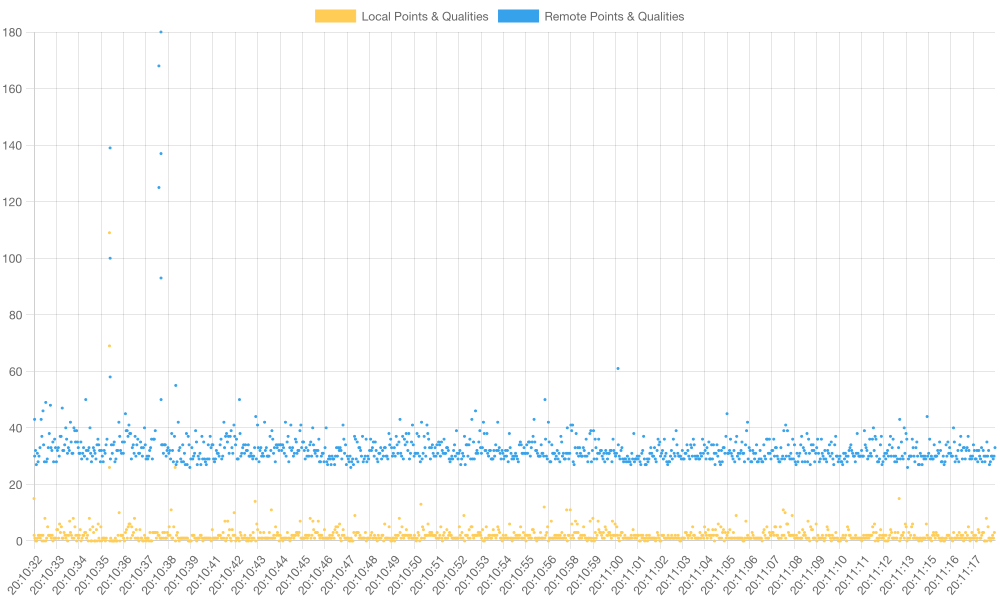
\includegraphics[scale=0.5]{04_Artefakte/01_Abbildungen/latency-65958016bcc0ee71c16f7fed}
\caption[Message latency on Computer A]{Latency in milliseconds for local and remote messages\protect}
\label{fig:latencyComputerA}
\end{figure}

\begin{figure}[h]
\centering
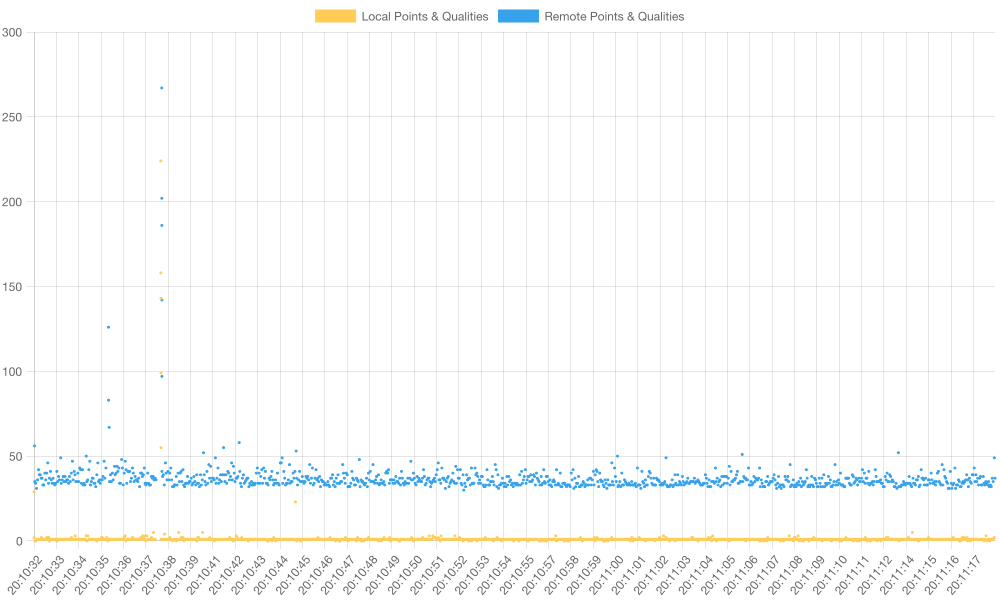
\includegraphics[scale=0.5]{04_Artefakte/01_Abbildungen/latency-65958034538b4baca4eb638a}
\caption[Message latency on Computer B]{Latency in milliseconds for local and remote messages\protect}
\label{fig:latencyComputerB}
\end{figure}

\subsection{Time spent}

\begin{figure}[h]
\centering
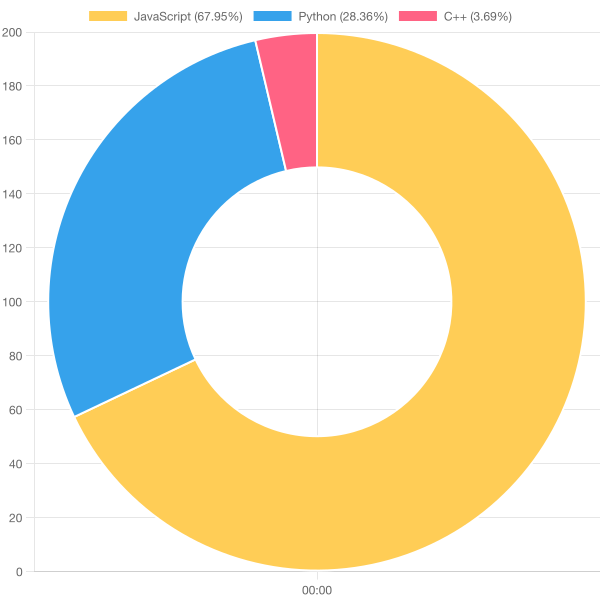
\includegraphics[scale=0.5]{04_Artefakte/01_Abbildungen/time-spent-on-languages}
\caption[Time spent on languages]{Time spent on various programming languages\protect}
\label{fig:timeSpentLanguages}
\end{figure}

\begin{figure}[h]
\centering
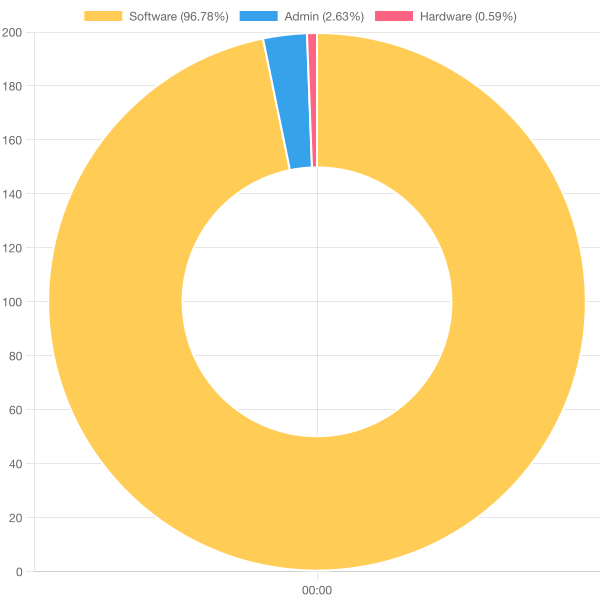
\includegraphics[scale=0.5]{04_Artefakte/01_Abbildungen/time-spent-on-types-of-work}
\caption[Time spent on areas of work]{Time spent on areas of work\protect}
\label{fig:timeSpentTypeOfWork}
\end{figure}


\subsection{Code quality}

\begin{figure}[h]
\centering
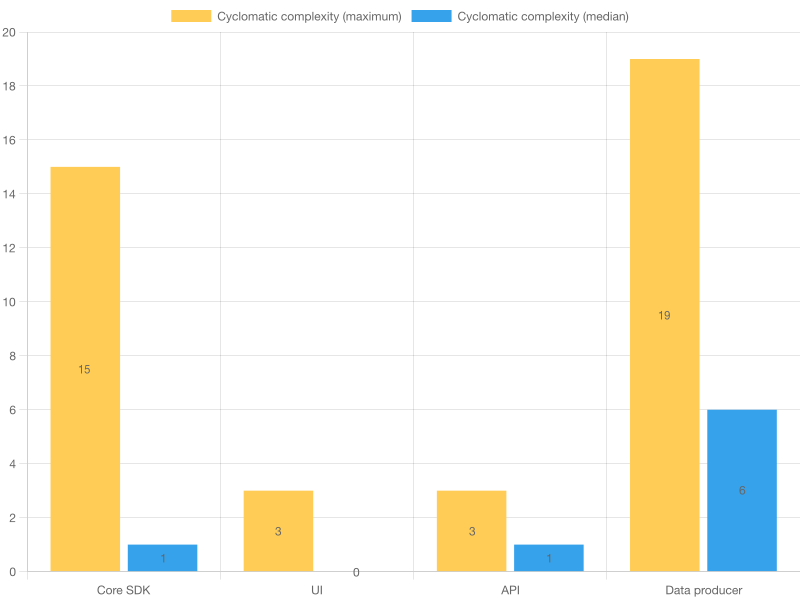
\includegraphics[scale=0.5]{04_Artefakte/01_Abbildungen/code-stats-complexity}
\caption[Cyclomatic complexity]{Cyclomatic complexity per component\protect}
\label{fig:cyclomaticComplexity}
\end{figure}

\begin{figure}[h]
\centering
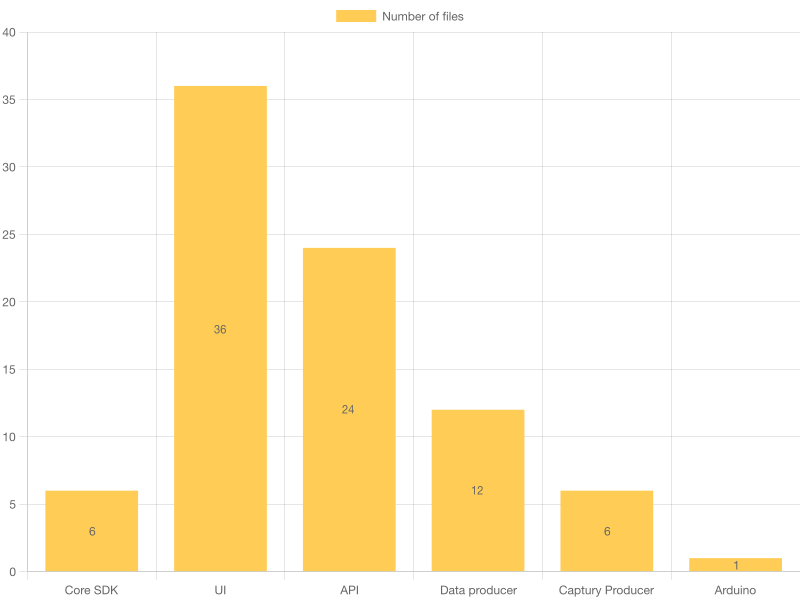
\includegraphics[scale=0.5]{04_Artefakte/01_Abbildungen/code-stats-filecount}
\caption[File count]{Number of source files per application component\protect}
\label{fig:fileCount}
\end{figure}

\begin{figure}[h]
\centering
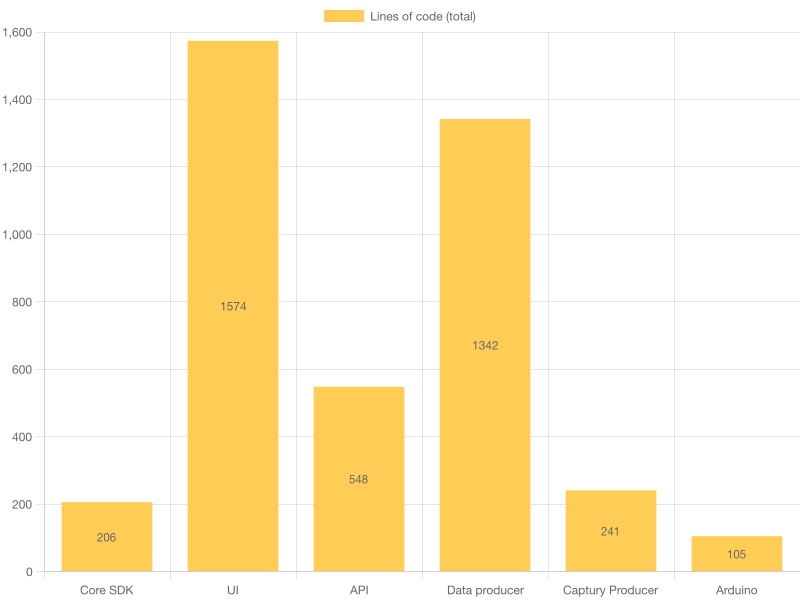
\includegraphics[scale=0.5]{04_Artefakte/01_Abbildungen/code-stats-loc-total}
\caption[Lines of code (total)]{Total lines of code per application component\protect}
\label{fig:linesOfCodeTotal}
\end{figure}

\begin{figure}[h]
\centering
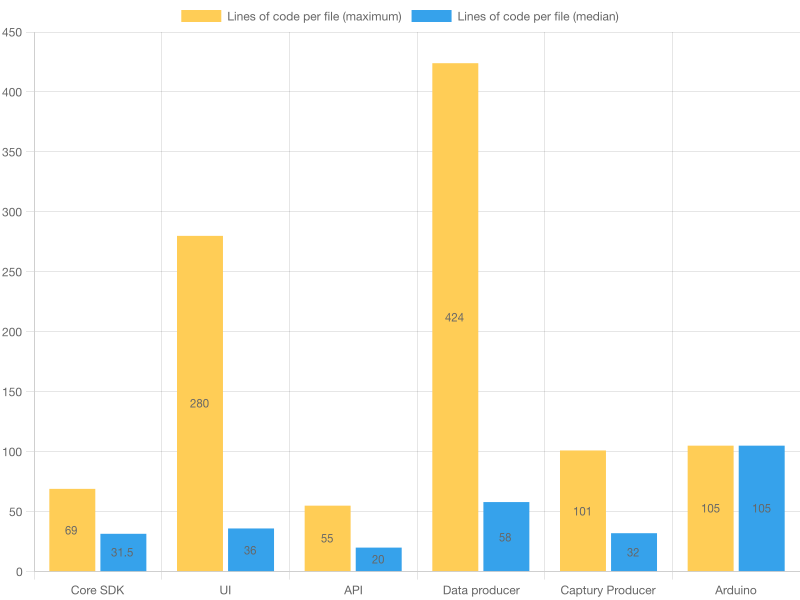
\includegraphics[scale=0.5]{04_Artefakte/01_Abbildungen/code-stats-loc}
\caption[Lines of code]{Maximum and median number of lines of code per application component\protect}
\label{fig:linesOfCode}
\end{figure}

\section{Critical reflection}
\label{sec:critical-reflection}

\subsection{Development process}

The development process was carried out in two main timeframes (X and Y) and followed the guiding principles decided in the concept.
It was a mostly pleasant experience with the selected frameworks delivering on their promised functionality and ease of use.
The initial setup was extremely quick due to the ease of setup of the WebRTC server and the quick generation of boilerplate code for the \ac{API} and the \ac{UI}.
However, the web audio standard implementation leaves a lot to desire, especially the support for spatial audio in the browser.
Currently, there is no built-in way to load custom \ac{HRTF} data, which should drastically improve the accuracy of spatial positioning for sound.
There are approaches using a custom build of the Chromium browser~\parencite{chromiumCustomHrtf} or a custom audio node~\parencite{customHrtfAudioNode} which unfortunately does not work with the \ac{SOFA} file format, so it is generally rather disappointing not seeing this thoroughly implemented in the general standard \ac{API}.

The initial setup for the data producers was also relatively quick, due to the large number of examples for the DepthAI \ac{SDK} and the clarity and hands-on approach to the main Python documentation.
The only thing lacking here, was a straightforward way to manage dependencies, as there were different results for the same dependencies being installed via PIP or Conda.

